\chapter{Polar Codes Background} \label{chap:PolarCodesIn5G}

\setcounter{secnumdepth}{3}
\renewcommand{\thesubsubsection}{\Alph{subsubsection}}

%\titleformat{\subsubsection}
%{\selectfont}{\thesubsubsection}{1em}{}

%Give background about polar codes and their adoption in 5G.
\paragraph{}
Polar codes were introduced by Arikan in his seminal work \cite{Arikan}. Polar codes are the class of capacity achieving codes. In the past decade, polar codes have sparked a interest from both academia and industrial resulting in significant research work in improving performance. The 5\textsuperscript{th} generation wireless systems (5G)  standardization has adopted polar codes for uplink and downlink control information for the enhanced mobile broadband (eMBB). Polar codes are also considered as the potential coding schemes for two other frameworks of 5G, namely ultra-reliable-low-latency (URLLC) and massive machine-type communications (mMTC).
\paragraph{}
Polar codes achieve capacity asymptotically for of memoryless channel. Although polar codes are the first theoretically capacity achieving codes with an explicit construction, capacity is approached only asymptotically their performance is suboptimal compared to LDPC or Turbo codes at short block lengths with successive cancellation decoding (SCD). \cite{TalVardy} Presents the improved version of SCD called \emph{successive cancellation list decoder(SCLD)}.
\paragraph{}
The construction of polar codes involves the identification of channel reliability values, information bits are placed in the K high reliable bit indices out of N positions and remaining bits are set to zero then these N bits are passed through a polar encoding circuit to get the encoded bits. Selection is of reliability indices is done based on the code length and channel signal-to-noise ratio. Due to varying code length and channel conditions in 5G systems significant effort has been put to identify reliability indices which have good error correction performance over multiple code length and channel parameters.

\section{Preliminaries} 
\paragraph{}
This section introduces the basic mathematical foundations of the polar codes. In particular, about the frozen set design, encoding and decoding. Different decoding algorithms are introduced. Mainly Successive Cancellation Decoding(SCD), Successive Cancellation List Decoding(SCLD) and CRC aided Successive Cancellation List Decoding(CA-SCLD). Examples of encoding and decoding with different algorithms are presented for better understanding.

\subsection{Polar codes definition} \label{polarCodesDefn}
\paragraph{}
Mathematical foundations of polar codes lay on the polarization effect of the matrix \cite{Arikan}. $ k = \begin{smallmatrix} 1 & 0 \\ 1 & 1 \end{smallmatrix}$ also called Arikan matrix. Polar codes are $(N,K)$ linear block codes of size $N = 2^{n}$ where $n$ being a natural number. $N$ is the block length of the code and $K$ is the number of information bits.  $N$-bit vector $U$ contains $K$ information and $N-K$ frozen bits which are set to known value mostly zeros. These bits are then multiplied with the generator matrix constructed from Kronecker power of Arikan kernel matrix.

For example $n=3$, block length $N$ becomes $8$ hence the generator matrix is \newline

$ k^{\otimes 3} = \begin{bmatrix}
1 & 0 & 0 & 0 & 0 & 0 & 0 & 0\\ 
1 & 1 & 0 & 0 & 0 & 0 & 0 & 0\\ 
1 & 0 & 1 & 0 & 0 & 0 & 0 & 0\\ 
1 & 1 & 1 & 1 & 0 & 0 & 0 & 0\\ 
1 & 0 & 0 & 0 & 1 & 0 & 0 & 0\\ 
1 & 1 & 0 & 0 & 1 & 1 & 0 & 0\\ 
1 & 0 & 1 & 0 & 1 & 0 & 1 & 0\\ 
1 & 1 & 1 & 1 & 1 & 1 & 1 & 1
\end{bmatrix}$ \newline

where $k^{\otimes n}$ denotes the $n^{th}$ Kronecker power of $k$. The encoding process involves the multiplication of $N$-bit vector $U$ consisting of $K$ information bits and $N-K$ frozen bits with $k^{\otimes n}$.

\subsubsection{Polar code construction} \label{CodeConstruction}
\paragraph{}
In polar coding, first step is to identify the channel reliability values for a particular block length, this step is also called as polar code construction. Basic idea of polar coding is to manufacture out of $N$ independent copies of given binary discrete memoryless channel create a fraction of channels which are either completely noiseless or noisy.This process of creating extremal channels is called channel polarization. As $N\to\infty$ fraction of noiseless channels approaches capacity of channel. Estimating reliability indices channels is carried by considering the Bhattacharyya parameter which indicates the reliability of individual channel.
 
\paragraph{}
For a generic binary-input discrete memoryless channel (B-DMC) which is represented as $W \colon \mathcal{X} \to \mathcal{Y}$ with input alphabet $\mathcal{X}$, output alphabet $\mathcal{Y}$ and transition probabilities given by $W(y|x),x \in \mathcal{X}, y \in \mathcal{Y}$.

Bhattacharyya parameter is given by 
\begin{equation}
	Z(W) \triangleq \sum_{y \in \mathcal{Y}} \sqrt{W(y|0)W(y|1)}
\end{equation}

Bhattacharyya parameter indicates how unreliable the channel is, It is easy see that $Z(W)$ takes values between $[0,1]$ better the channel smaller is $Z(W)$. Polarization creates channels with $Z(W)$ 0 or 1.

\textbf{Here Give one example channel polarization for BEC channel and show the evolution of channel reliabilities. May include a insert a picture with evolution of channel reliabilities plot.}


\subsubsection{Encoding}
As explained in the section \ref{CodeConstruction} code construction is done. Information bits are placed in the most reliable bit indices position non reliable bit positions are called frozen bits whose values are set to zeros. This $N$-bit vector $U$ is multiplied with generator matrix obtained by the Kronecker power of Arikan kernel matrix. Multiplying with generator matrix can also be represented as circuit form. for $n = 3$ block length $N$ becomes 8 for such a case encoding circuit looks as shown in the following figure. \newline


\begin{figure}[!htb]
	\centering
	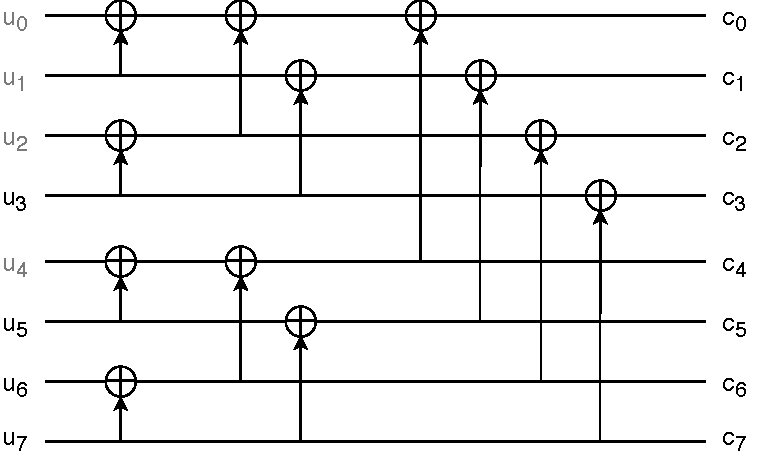
\includegraphics[width=0.8\textwidth]{./figures/EncodingCircuit.pdf}
	\caption{Polar encoder in circuit form for $N = 8$}
	\label{fig:encoderCircuit}
\end{figure}

the grayed locations are the frozen bit indices which are set to zero, in remaining positions information bits are inserted. Output of the circuit is a code word which is transmitted over the channel.

Lets consider an example with $N = 8$ and $K = 4$, rate of this code is $R = K/N = 1/2$. As given in the figure frozen bit indices are ${\{0,1,2,4\}}$ remaining indices contain information bits.  Let the infomation which needs to transmitted be \{1,1,0,0\}, then after placing information bits at reliable channel positions the vector $U$ becomes \{0,0,0,1,0,1,0,0\}






